%\documentclass[10pt]{beamer}
%\usetheme{amcg}

%\begin{document}

\section{Water collapse}

\frame{
  \frametitle{Water collapse}
  \begin{itemize}
    \item Fluidity is used to replicate a laboratory experiment of a collapsing column of water within an atmosphere of air (Lakehal et al., 2002).\newline
    \item A reservoir of water is initially held behind a barrier.\newline
    \item The water column collapses and floods the rest of the tank when the barrier is quickly removed.
  \end{itemize}
}

\frame{
  \frametitle{Water collapse - Simulation setup}
  \begin{itemize}
    \item The multi-material approach is used to represent the two fluids.
    \item The flow is assumed to be incompressible, inviscid, and 2D.
    \item Free-slip boundary conditions on the bottom and sides, and open top.
  \end{itemize}
        \hspace{-.05\textwidth}
 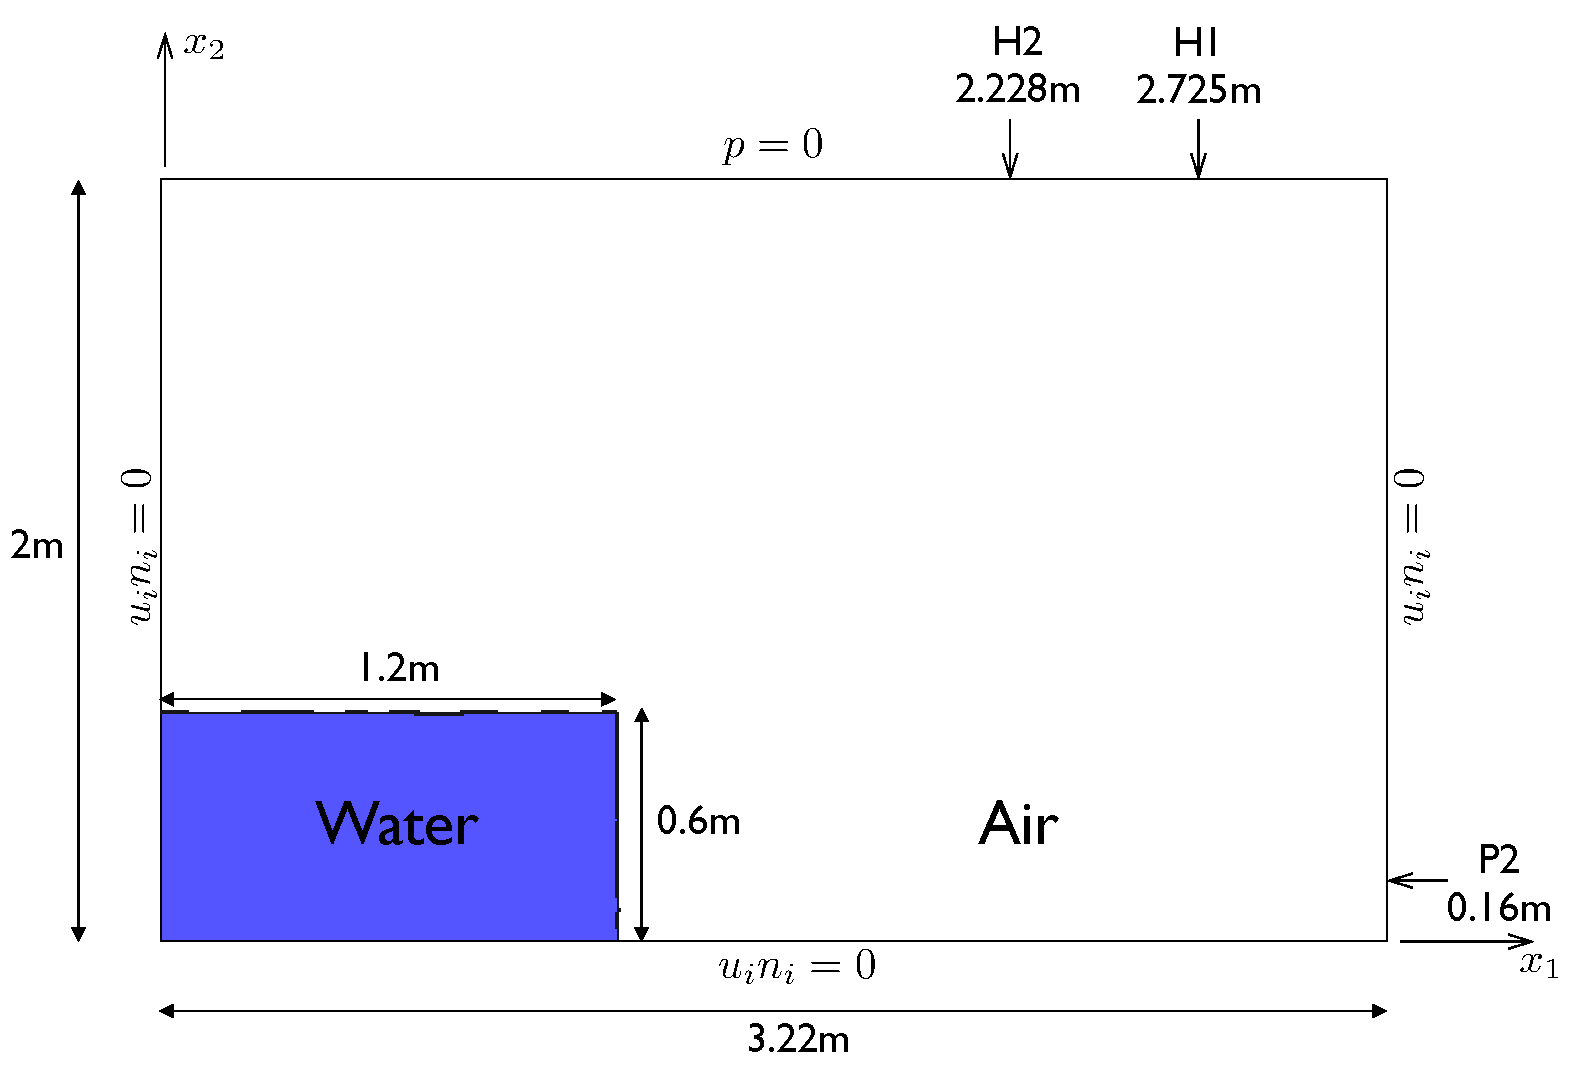
\includegraphics[scale=0.23]{./water_collapse/setup1.pdf}
 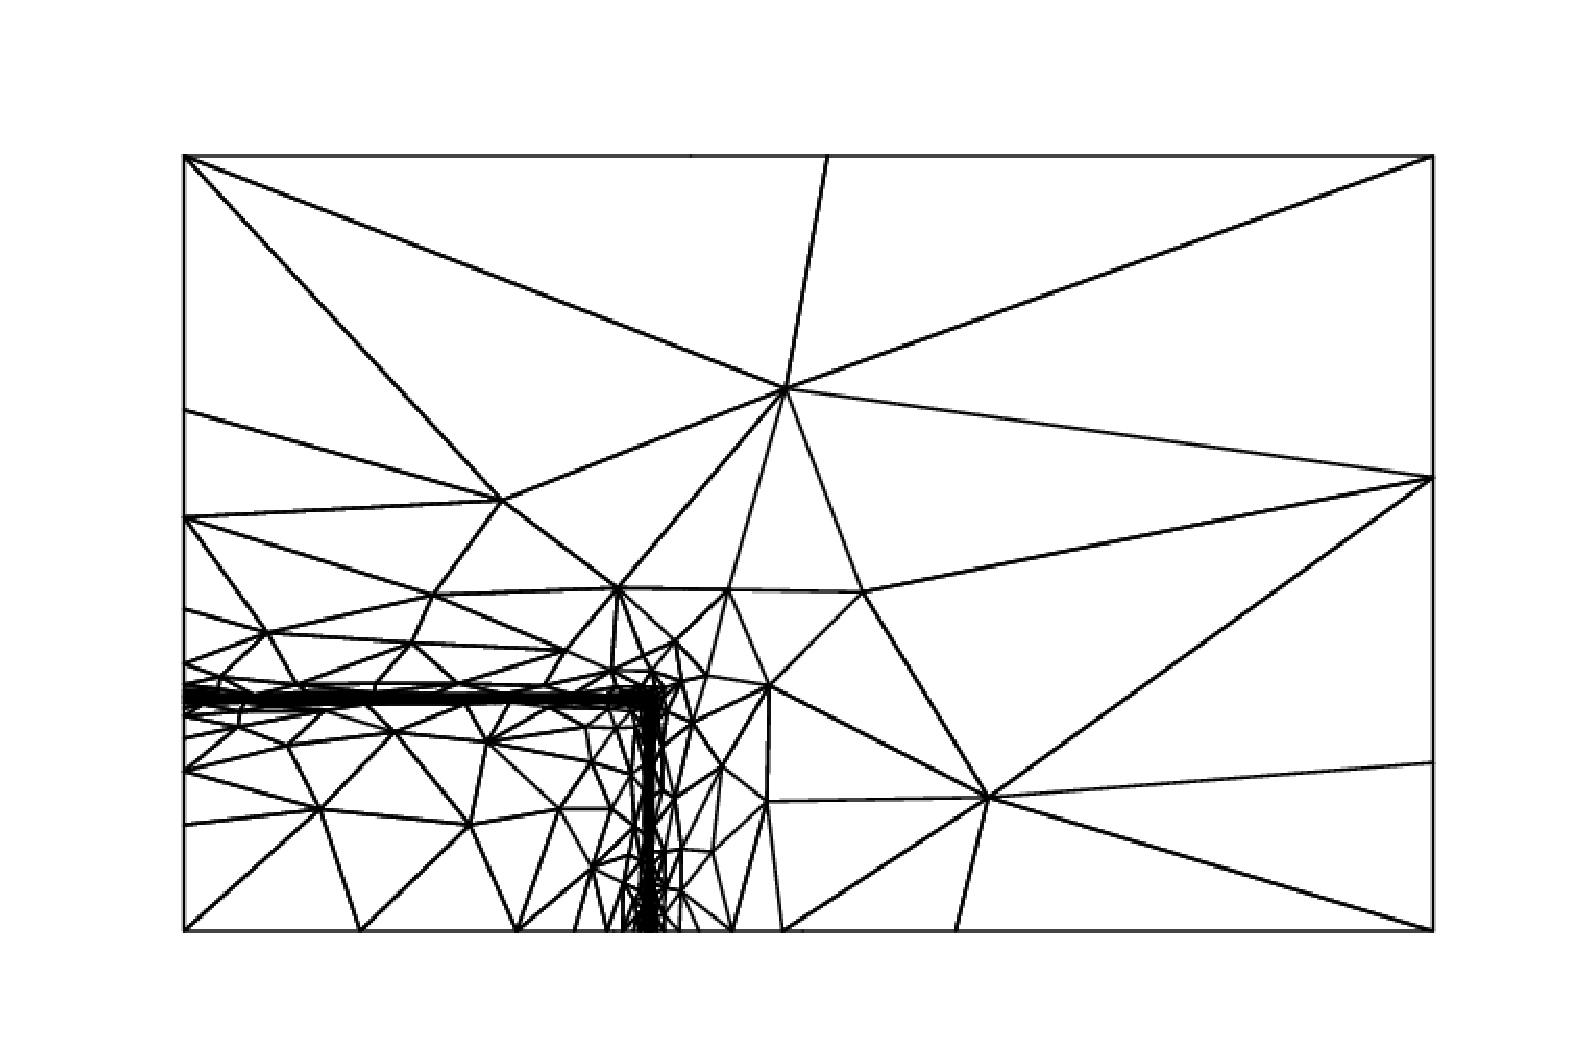
\includegraphics[scale=0.23]{./water_collapse/setup2.pdf}
}

\frame{
  \frametitle{Water collapse - Numerical results (1)}
\begin{figure}[H]
        \centering
 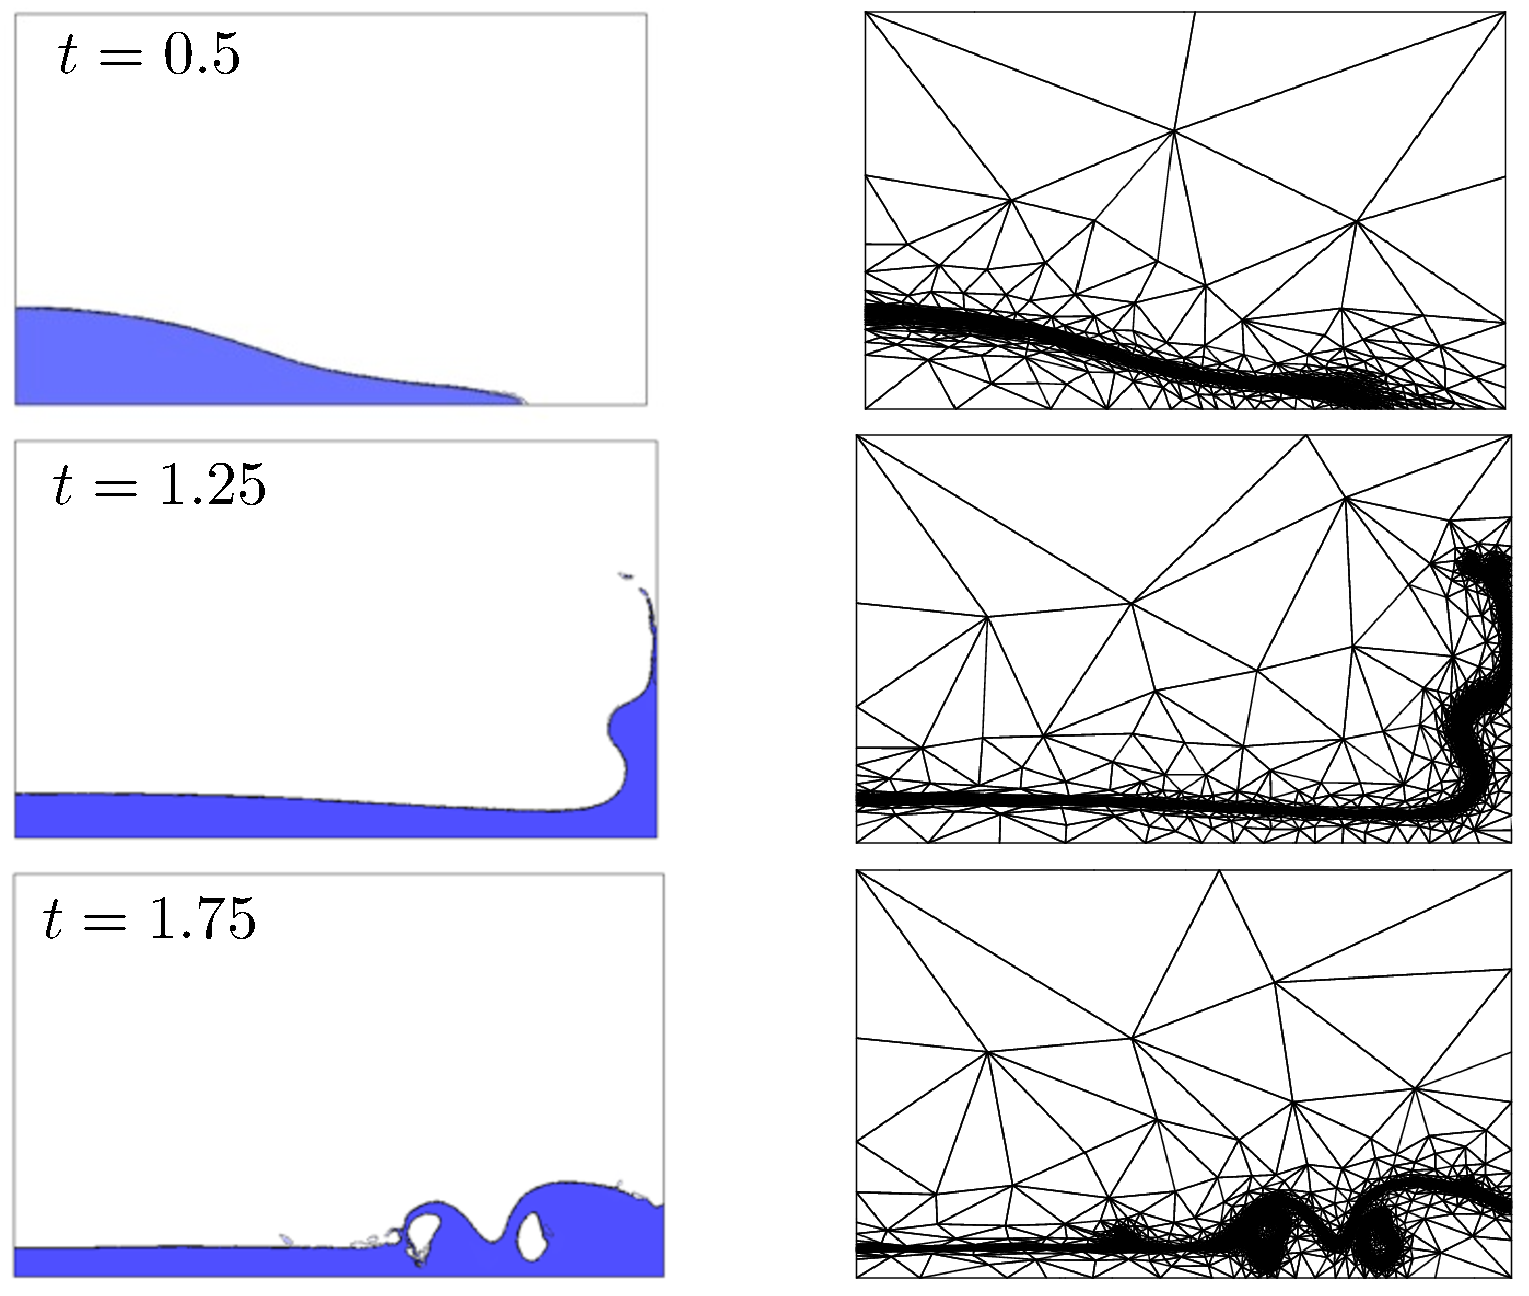
\includegraphics[scale=0.28]{./water_collapse/results1.pdf}
\end{figure}
}

\frame{
  \frametitle{Water collapse - Numerical results (2)}
        \vspace{-.025\textwidth}  
\begin{figure}[H]
        \centering
  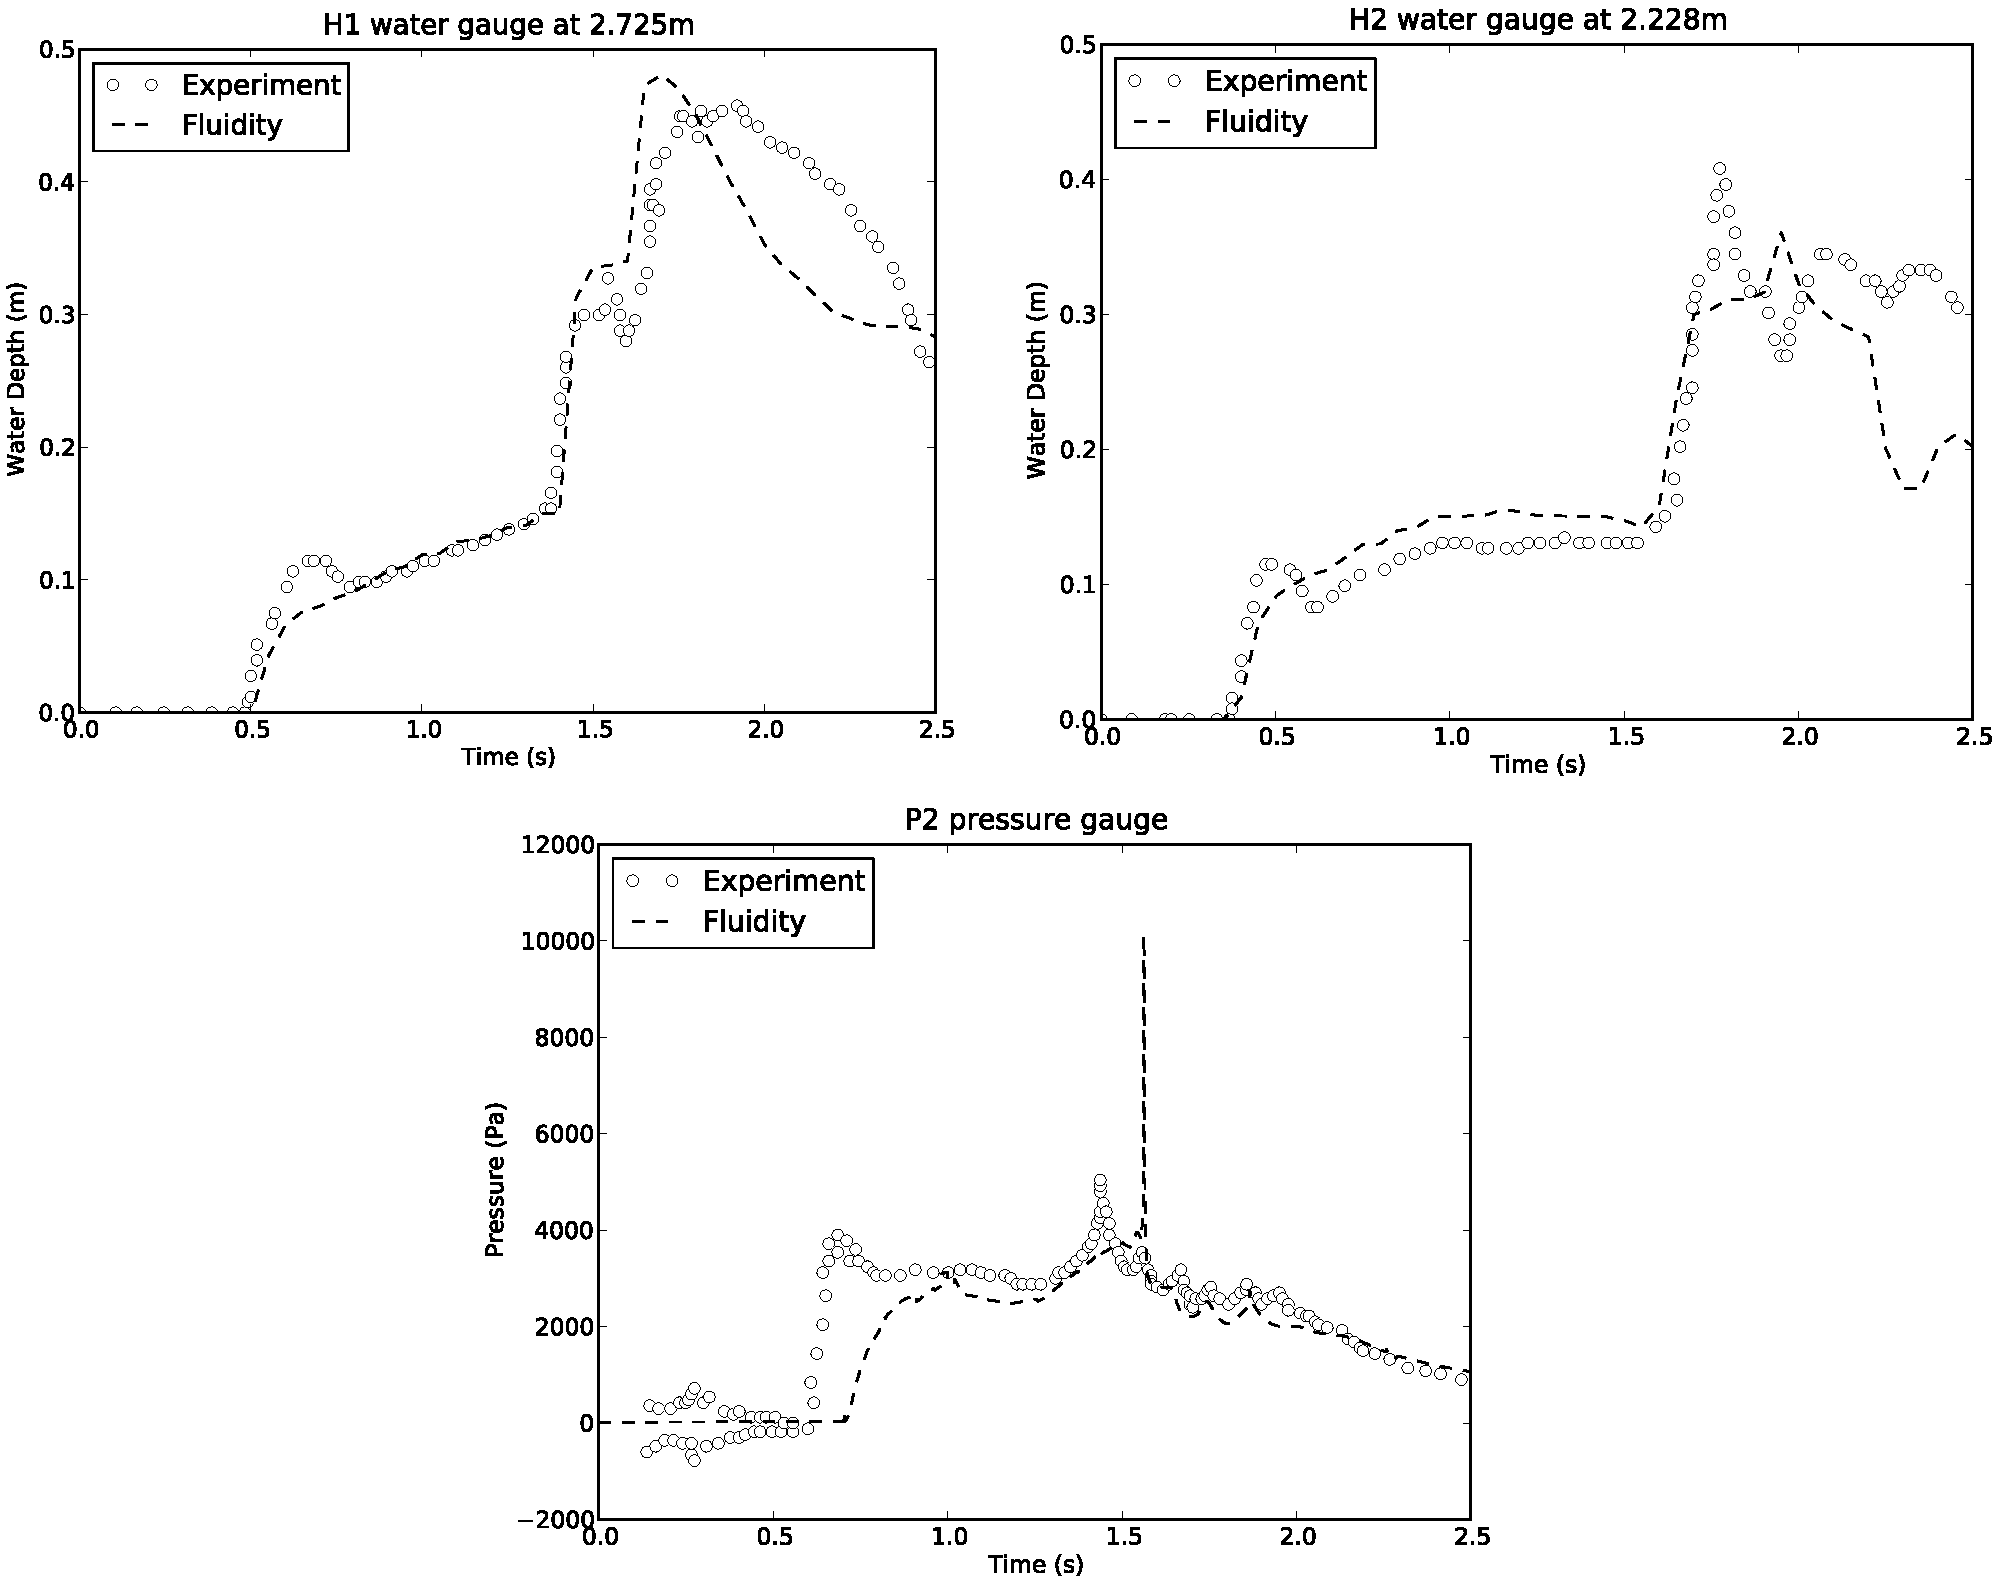
\includegraphics[scale=0.25]{./water_collapse/results2.pdf}
\end{figure}
}

\frame{
  \frametitle{Water collapse - Exercises}
 \begin{itemize}
    \item Disable the adaptivity option to run on a fixed mesh.\newline
    \item Alter the water/air viscosity/density.\newline
    \item Modify the tank geometry.
 \end{itemize}
}

%\end{document}
